\begin{flalign*}
& \v q = 0 \text{ --- положение равновесия} &\\
& T = \frac{1}{2}(A(q)\dv q, \dv q) \quad \Pi = \Pi(0) + \left( \left.\pd{\Pi}{\v q}\right|_{\v q = 0}, \v q \right) + \frac{1}{2}\left(\left.\pd{^2 \Pi}{\v q^2}\right|_{\v q = 0}, \v q \right) + \ldots = \Pi^{(0)} + \Pi^{(1)} + \Pi^{(2)} + \ldots &\\
& \Pi^{(0)} = \Pi(0) = 0, \; \Pi^{(1)} = \left( \left.\pd{\Pi}{\v q}\right|_{\v q = 0}, \v q \right) = 0 &\\
& \Pi^{(m)} \text{ --- первая нетривиальная форма } \Pi &\\
\end{flalign*}

\begin{xmp}
\begin{enumerate}
\item $\Pi(x, y) = \frac{x^4 + y^4}{2}, \quad x = y = 0 \text{ --- устойчивое положение равновесия.}$
\item \begin{flalign*}
& T = \frac{\dot x^2 + \dot y^2}{2} \quad \Pi(x, y) = \frac{x^2}{2} \quad \Pi^{(2)} = \frac{x^2}{2} &\\
& \frac{d}{dt} \pd{T}{\dot x} - \pd{T}{x} + \pd{\Pi}{x} = \ddot x + x = 0 &\\
& \frac{d}{dt} \pd{T}{\dot y} - \pd{T}{y} + \pd{\Pi}{y} = \ddot y = 0 \qquad y = ct + c_1&\\
& x = y = 0 \text{ --- неустойчивое положение равновесия.} &\\
\end{flalign*}
\end{enumerate}
\end{xmp}

\begin{teo}
Если $\Pi$ не имеет даже нестрогого минимума в окрестности некоторого положения равновесия натуральной системы, то равновесие неустойчиво.
\end{teo}

\begin{teo}
\begin{flalign*}
& \underline{m = 2, n = 1}: T = \frac{1}{2}a(q)q^2, \; a(q) > 0 &\\
& b = \left.\pd{^2 \Pi}{q^2} \right|_{q = 0} < 0 &\\
& L = \frac{1}{2}a(q)\dot q^2 - \frac{1}{2}bq^2 + O_3(q) &\\
& 0 = \frac{d}{dt}\pd{L}{\dot q} - \pd{L}{q} = a(q)\ddot q + a'_q \dot q^2 - \frac{1}{2}a'_q \cdot \dot q^2 + bq + O_2(q) = &\\
& = a(q)\cdot \ddot q + bq + O_2(q, \dot q) &\\
&
\begin{cases}
\frac{d}{dt}q = \dot q \\
\frac{d}{dt}\dot q = - \frac{bq - O_2(q, \dot q)}{a(0) + O_1(q)} = -\frac{bq}{a(0)} + \cancel{O_2(q, \dot q)} \\
\end{cases} &\\
& \v x = (q, \dot q)^T, \; \dv x = A\v x &\\
& A = \left( \begin{matrix}
0 & 1 \\
- \frac{b}{a(0)} & 0 \\
\end{matrix} \right) &\\
& \det(A - \lambda E) = \lambda^2 + \frac{b}{a(0)} = 0 \Leftrightarrow \lambda^2 = - \frac{b}{a(0)} > 0 &\\
& \lambda = \pm \sqrt{-\frac{b}{a(0)}} &\\
& \re \lambda_+ > 0 \Rightarrow q = 0 \text{ --- неустойчивое положение равновесия.}
\end{flalign*}
\end{teo}

\begin{ntc}
\begin{flalign*}
& L = \underbrace{\frac{1}{2}a(t)q^2 - \frac{1}{2}bq^2}_{L^*} + O_3(q, \dot q) &\\
& C = \left.\pd{^2 \Pi}{q^2}\right|_{q = 0} &\\
& C \text{ --- положительно определена} \Rightarrow q = 0 \text{ --- устойчиво} &\\
& \det C = 0 \text{ --- } ? &\\
& \exists \Delta_i < 0 &\\
\end{flalign*}
\end{ntc}

\subsection{Влияние гироскопических и диссипативных сил на устойчивость равновесия}
\begin{flalign*}
& \frac{d}{dt}\pd{L}{\dv q} - \pd{L}{\v q} = Q^* &\\
& L = \frac{1}{2}(A(q)\dv q, \dv q) - \Pi(q) &\\
& \dot E = (\v Q^*, \dv q)  \qquad E = T + P &\\
\end{flalign*}

\begin{itemize}
\item Если $(\v Q^*,\; \dv q) = 0$, то $\v Q^*$ --- гироскопическая.
\item Если $(\v Q^*,\; \dv q) \leqslant 0$, то $\v Q^*$ --- диссипативная.
\item Если $(\v Q^*,\; \dv q) < 0$, то $\v Q^*$ обладает полной диссипацией.
\end{itemize}

\begin{teo}[Кельвина-Четаева 1]
Если $q = 0$ --- точка строгого локального минимума $\Pi$ натуральной системы, то даже при добавлении в систему гироскопических и (или) диссипативных сил, она является устойчивым положением равновесия $A$. Если при этом диссипативные силы обладают полной диссипацией, то это равновесие устойчиво асимптотически.
\end{teo}
\begin{proof}
\begin{flalign*}
& V(\v q, \dv q) = T + \Pi(\v q) - \Pi(q) &\\
& q = 0 \text{ --- строгий локальный минимум } \Pi(q) \Rightarrow V(0, 0) = 0,\; V(\v q, \dv q) > 0 \quad \forall \v q, \dv q \; 0 < \norm{q}^2 + \norm{\dv q}^2 < \varepsilon &\\
& a) \dot V = (\v Q^*, \dv q) \leqslant 0 \Rightarrow q = 0 \text{ --- устойчиво по теореме Ляпунова} &\\
& b) \dot V = 0 \Leftrightarrow \dv q = 0 \Leftrightarrow q = 0 \Rightarrow q = 0 \text{ --- устойчиво асимптотически по т. Барабашина-Красовского} &\\
\end{flalign*}
\end{proof}

\begin{teo}[Кельвина-Четаева 2]
Если в изолированном положении равновесия $\Pi$ не имеет даже нестрогого минимума, а силы обладают полной диссипацией, то равновесие неустойчиво (вне зависимости от направления гироскопических сил).
\end{teo}
\begin{proof}
\begin{flalign*}
& V(\v q, \dv q) = T + \Pi(\v q) - \Pi(0) &\\
& q = 0 \text{ --- ...} \Rightarrow \Omega: \Pi(\v q) < \Pi(0) \; \forall q \in \Omega &\\
& \qquad \qquad \qquad \qquad \Pi(q) = \Pi(0) \; \forall q \in \partial \Omega, \; q = 0 \in \partial Q &\\
& V < 0, \dot V < 0 \quad \forall \{\v q, \dv q\} \in \Omega' = \{ \v q, \dv q : q \in \Omega, \dv q = 0 \} &\\
& \dot V = 0 \Leftrightarrow \v q = 0 &\\
& \Rightarrow q = 0 \text{ --- неустойчиво по теореме Красовского.}
\end{flalign*}
\end{proof}

\begin{xmp}
\begin{flalign*}
	& \ddot x = 0,\; x = 0 \text{ --- неустойчиво.} &\\
	& \ddot x = -k\dot x,\; k > 0 &\\
	& \lambda^2 + k\lambda = 0 \Rightarrow \begin{cases}
		\lambda = 0 \\
		\lambda = -k < 0 \\
	\end{cases}&\\
	& \ddot x = 0,\; x = 0 \text{ --- неустойчиво.} &\\
	& \ddot x = -k\dot x,\; k > 0 &\\
	& \lambda^2 + k\lambda = 0 \Rightarrow \begin{cases}
		\lambda = 0 \\
		\lambda = -k < 0 \\
	\end{cases}&\\
	& x = 0 \text{ --- устойчиво.} &\\
\end{flalign*}
\end{xmp}
\begin{xmp}[Гироскопическая стабильность]
	\begin{flalign*}
		& T = \frac{\dot x^2 + \dot y^2}{2} \qquad \Pi = -\frac{x^2 + y^2}{2} \qquad \v Q^* = 2 \dot y \v e_x - 2 \dot x \v e_y &\\
		& (\v Q^*,\dv q) = 2 \dot y\dot x - 2 \dot x\dot y = 0 &\\
		& \begin{cases}
			\ddot x - x = 2 \dot y \\
			\ddot y - y = -2 \dot x \\
		\end{cases} \qquad \left( \dv x = A\v x,\ \det(A - \lambda E) = 0 \right) &\\
		& A\ddot{\v x} + B\dv x + C \v x = 0 &\\
		& \det(A\lambda^2 + B\lambda + C) = 0 &\\
		& A = \left( \begin{matrix}
			1 & 0 \\
			0 & 1 \\
		\end{matrix} \right) \qquad B = \left( \begin{matrix}
			0 & -2 \\
			2 & 0 \\
		\end{matrix} \right) \qquad C = \left( \begin{matrix}
			-1 & 0 \\
			0 & -1 \\
		\end{matrix} \right) &\\
		& \det(A\lambda^2 + B\lambda + C) = \begin{vmatrix}
			\lambda^2 - 1 & -2\lambda \\
			2\lambda & \lambda^2 - 1 \\
		\end{vmatrix} = \lambda^4 - 2\lambda^2 + 1 + 2 ^2\lambda^2 &\\
		& \left[ \begin{array}{l}
			\lambda^2 = -2 \\
			\lambda^2 = -\frac{1}{2} \\
		\end{array} \right. \qquad \begin{array}{l}
			\lambda = \pm \sqrt 2 i \\
			\lambda = \pm \frac{\sqrt 2}{2}i \\
		\end{array} &\\
		& x = y = 0 \text{ --- устойчивое.} &\\
	\end{flalign*}
\end{xmp}

\subsection{Элементы теории бифуркации}
\begin{flalign*}
& \dv x = \v f(\v x, \alpha),\; \v x \in \R^{n},\; \alpha \in \R^n &\\
& \text{Кривые равновесий } \v x = \v x(\alpha): \v f(\v x(\alpha), \alpha) = 0 &\\
& \text{Точка бифуркации } (\v x_*, \alpha_*): \left.\pd{\v f}{\v x} \right|_{\v x = \v x^*(\alpha_*), \; \alpha = \alpha_*} = 0
\end{flalign*}

\begin{figure}[H]
	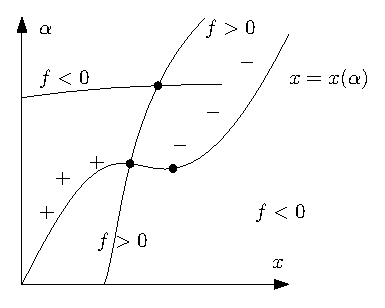
\includegraphics{4_1.eps}
\end{figure}
\begin{flalign*}
	& \underline{n = 1}\quad \dot x = f(x,\;\alpha) &\\
	& \dot x = f'_x(x - x(\alpha)) + O_2(x - x(\alpha)) &\\
	& \lambda = f_x' > 0 \Rightarrow x = x(\alpha) \text{ --- неустойчиво.} &\\
	& \lambda = f_x' < 0 \Rightarrow x = x(\alpha) \text{ --- устойчиво.} &\\
	& \lambda = f_x' = 0 \Rightarrow \text{бифуркация.} &\\
\end{flalign*}
\subsubsection*{Основные типы бифуркаций.}
\begin{figure}[H]
	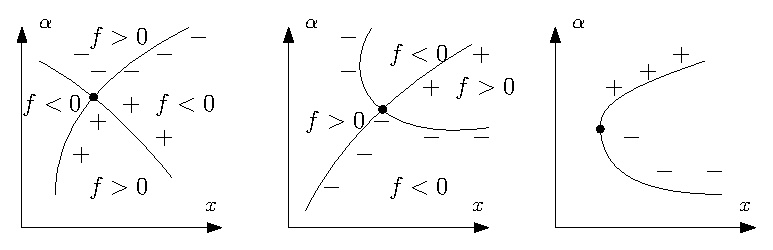
\includegraphics{4_2.eps}
	\caption*{1) Смена устойчивости, 2) вилка, 3) складка.}
\end{figure}
\begin{flalign*}
	& \frac{d}{dt}\pd{L}{\dv q} - \pd{L}{\v q} = 0 \qquad L = \frac{1}{2}\left( A(q)\dv q,\; \dv q \right) - \Pi(\v q,\; \alpha) &\\
	& \text{Кривая равновесия } \left.\pd{\Pi}{\v q}\right|_{\v q = \v q(\alpha)} = 0 &\\
	& \text{Точка бифуркации } \det\left( \left.\pd{^2 \Pi}{\v q^2}\right|_{\v q_* = \v q(\alpha_*), \alpha = \alpha_*} \right) = 0 &\\
	& \underline{n = 1}\quad a\ddot q + bq = 0,\; b = \pd{^2 \Gamma}{q^2} &\\
	& a\lambda^2 + b = 0 &\\
	& \lambda^2 = -\frac{b}{a} &\\
	& 1) b > 0 \quad \lambda = \pm\sqrt{\frac{b}{a}}i \text{ --- устойчиво.} &\\
	& 2) b < 0 \quad \lambda = \pm \sqrt{-\frac{b}{a}} \text{ --- неустойчиво.} &\\
	& \text{Равновесия: } \left[\begin{array}{l}
		\varphi = 0 \\
		\varphi = \pi \\
		\varphi = \pm \arccos \frac{g}{\omega^2r} \\
	\end{array}\right.
\end{flalign*}
\begin{figure}[H]
	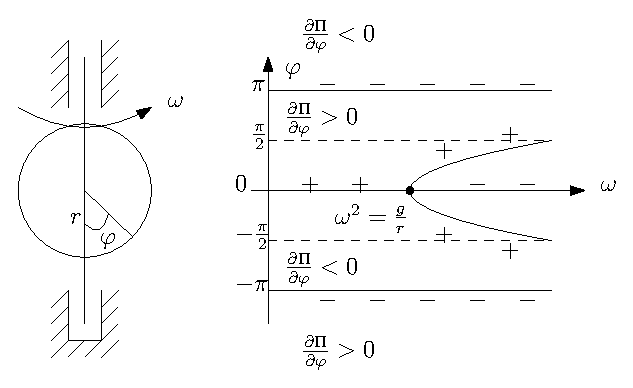
\includegraphics{4_3.eps}
\end{figure}